% !TEX root = omar-thesis-proposal.tex
\section{Motivation}\label{motivation}\begin{figure}
\begin{center}
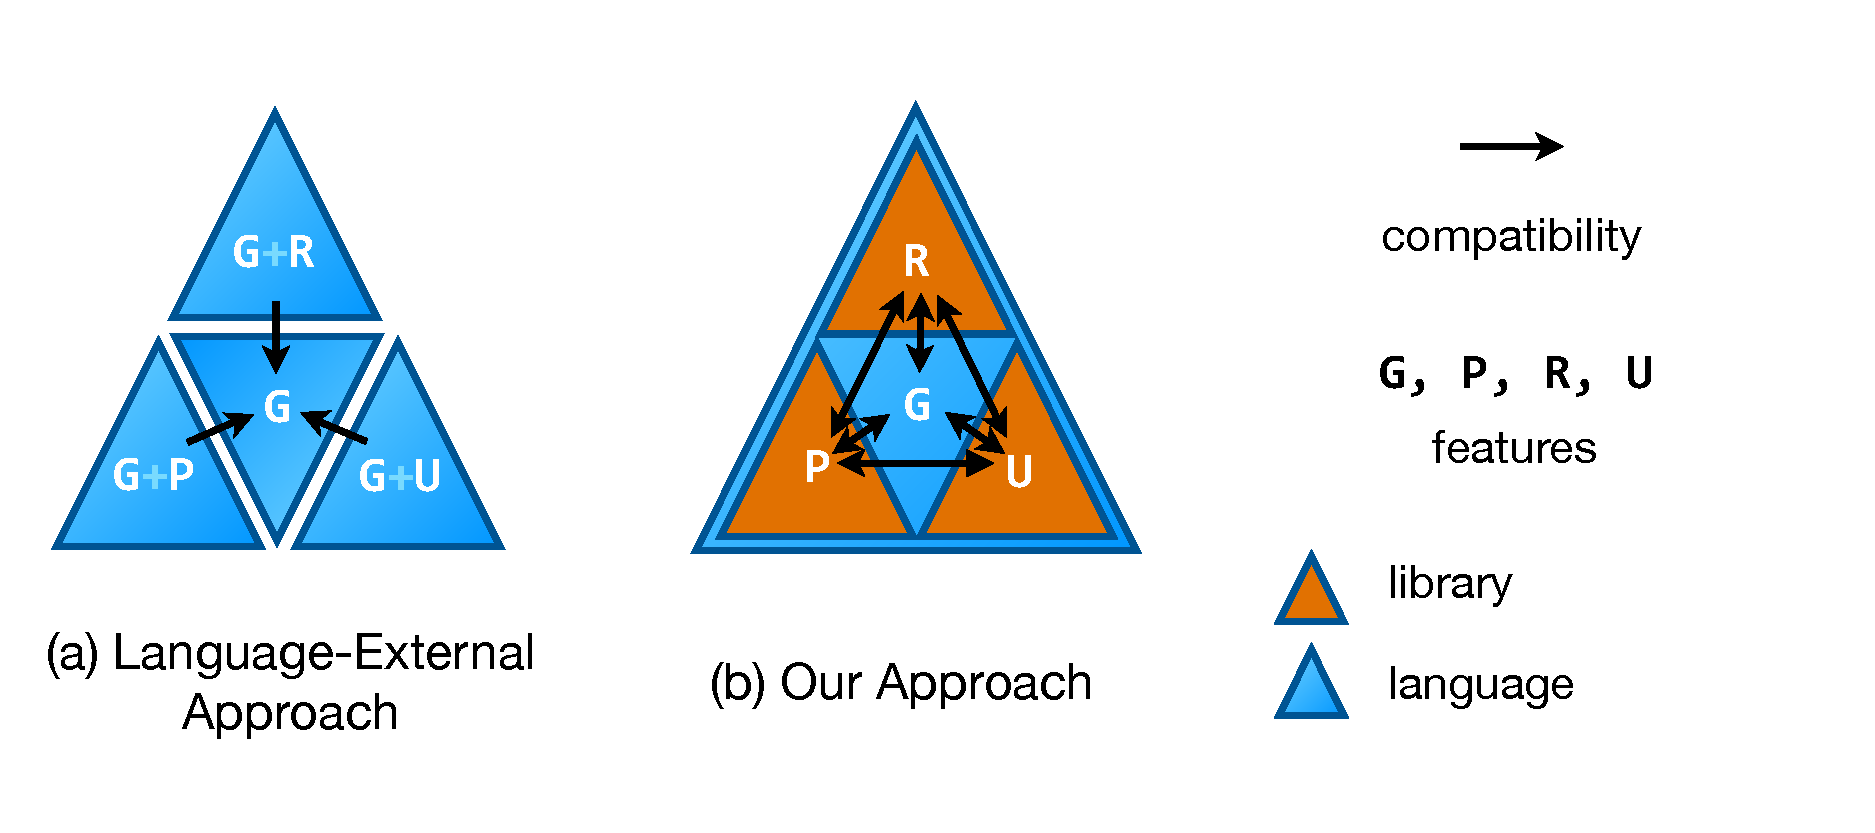
\includegraphics[scale=0.45]{approaches.pdf}
\end{center}
\vspace{-20px}
\caption{\small (a) With the language-external approach, novel constructs are packaged into separate languages. Users can only safely and naturally call into languages if the interface uses common constructs and an interoperability layer has been developed (the \emph{interoperability problem}). (b) With the language-internal approach, there is one extensible host language and the compile-time and edit-time logic governing novel constructs is expressed within libraries. If the extension mechanism guarantees the safety of arbitrary compositions of extensions, the necessary primitives can simply be imported by library clients as needed, and so interoperability is not a problem.}
\label{approaches}
\end{figure}
Designing and implementing a programming language together with its supporting tools (collectively, a \emph{programming system}) that has a sound theoretical foundation, helps users identify and fix errors as early as possible, supports a natural programming style, and that performs well across diverse problem domains and hardware platforms remains a grand challenge in computing. It has become clear that no small, fixed collection of primitive abstractions and tools can fully satisfy these criteria in all situations. Rather, researchers and domain experts must continue, in a principled manner, to design and implement novel abstractions, provide alternative implementations of existing abstractions, and supplement languages with new tools, and tools with new behaviors, to better satisfy these criteria within the constraints of different problem domains. 

%To realize a new abstraction or system behavior, such experts can consider either a \emph{language-internal approach}, where they work within an existing language and distribute their solutions as libraries, or a \emph{language-external approach}, where they create a new, distinct programming system (often centered around what has come to be called a new \emph{domain-specific language} \cite{dsl}) or extend an existing system by some mechanism that is not part of the language itself, such as an extension mechanism supported by a {particular} compiler, editor or other tool.

When possible, taking a \emph{language-internal approach} to implementing a new abstraction or system behavior (collectively, a new \emph{feature}) is simpler and more practical. If a feature can be realized by creatively repurposing existing features and distributed as a library, both providers and clients face fewer barriers to adoption because it is easy to gradually integrate library-based features into existing code and they leverage well-understood and well-developed mechanisms. But taking this approach is often \emph{not} possible today because libraries are generally vehicles for specifying the run-time behavior of a program. The compile-time and edit-time behaviors of a programming system cannot easily be adapted or extended in a specialized way from within libraries in most programming systems. That is, the language's syntax, static semantics and corresponding dynamic semantics are fixed in advance, the compiler is a ``black box'' implementation of these fixed semantics, and the other tools, like code editors and debuggers, operate according to fixed, domain-agnostic protocols based on these fixed semantics.

If any of these components of the system must be modified to realize a new feature, providers must instead take a \emph{language-external approach}, either by developing a new or derivative programming system (often centered around a so-called \emph{domain-specific language} \cite{dsl}) or by extending an existing system by some mechanism that is not part of the language itself, such as an extension mechanism supported by a {particular} compiler or other tool. %Extending a particular tool is morally equivalent, for our purposes, to creating a new system, because we aim to minimize the extent to which the edit-time, compile-time and run-time semantics of libraries depend on the implementation details of a particular tools.

Unfortunately, when providers of new features take language-external approaches, it causes problems for clients. Features become coupled to a collection of other unrelated and often underdeveloped features, making adoption more costly when these other choices are not appropriate. For example, although recent evidence suggests that developers prefer language-integrated parallel programming abstractions to library-based implementations if all else is equal \cite{langvslib}, library-based implementations remain more widely adopted because they do not require porting applications to a language designed around a few privileged parallel programming abstractions. These abstractions may only be useful in performance-critical portions of the application, and then only in cases where no competing abstraction would be more appropriate. 


%\item Developing a new language and its associated tools places a significant development burden on providers who may wish only to promote a few core innovations, although tools like compiler generators, language workbenches and easy-to-extend tools can decrease this burden. 
%\item 

%Clients seem to prioritize the ability to choose different features for different portions of an application. 
If it were easy to call between languages, then having a variety of specialized languages would be less of a problem. In fact, some have advocated for just this development model, calling it the the \emph{language-oriented approach} to software development \cite{languageoriented}. A fundamental problem with this approach, however, arises at the interfaces between languages. The specialized abstractions particular to one language cannot be safely and naturally expressed in another, in general, so building a program out of components written in many different languages is difficult or impossible whenever these specialized abstractions are exposed at library interface boundaries. We refer to this as the \emph{interoperability problem}. 

One strategy increasingly being taken by programming language designers to partially address the interoperability problem today is to target an established language, such as the Java Virtual Machine (JVM) bytecode, and support a superset of its constructs. Scala \cite{scala} and F\# \cite{fsharp} are examples of general-purpose languages that have taken this approach. This only provides full interoperability in one direction (Figure \ref{approaches}a). While calling into the common language becomes straightforward, calls in the other direction, or between the languages sharing the common target, are still restricted by the constructs available in the common language. If full interoperability is desired, new languages must only include constructs that can already be expressed safely and reasonably naturally in the common language. Many innovative features, however, can be difficult to define in terms of existing features in ways that guarantee all necessary invariants are maintained and that do not require large amounts of boilerplate code. For example, the type system of F\# guarantees that null values cannot occur within F\# data structures, but maintaining this important invariant still requires run-time checks because the typing rules of F\# do not apply when F\# code is called from other languages on the Common Language Infrastructure (CLI) like C\#. The F\# type system also includes support for checking that units of measure are used correctly \cite{fsharpunits}, but this domain-specific invariant is left completely unchecked at language boundaries. In Scala, interfaces built around traits that have default method implementations are difficult to implement from Java or other JVM languages and the workaround can break if the trait is modified \cite{scalatraitinterop}. In some cases, desirable features must be omitted entirely due to concerns about  interoperability. The module system in F\#, for example, is substantially simpler than that in its predecessor, OCaml, despite F\# otherwise aiming to maintain compatibility, due to the need for bidirectional interoperability between F\# and other CLI languages.
%\end{itemize}

For these reasons, we argue that the language-oriented approach is fundamentally flawed and so taking a language-external approach to realizing a new feature, where new features are packaged into mutually incompatible languages and associated tools, should be considered harmful and avoided when possible. The goal of the research proposed here is to fundamentally reorganize the core components of the programming system so that such language-external approaches are less frequently necessary, by designing \emph{language-internal extension mechanisms} that give developers control over edit-time and compile-time behaviors that have previously been centrally-controlled by  the  committees that govern languages or tools\footnote{One might compare today's monolithic programming systems to  {centrally-planned} economies, whereas extensible\- languages more closely resemble modern market economies.}\todo{read Arch D. Robison. Impact of economics on compiler optimization.}. Specifically, we will show how control over \textbf{parsing}, \textbf{typechecking}, \textbf{translation} (the first stage of compilation) and \textbf{code completion} can be delegated to user-defined logic distributed in {libraries}, as illustrated in Figure \ref{approaches}b. Such libraries are called \emph{active libraries} because, rather than being passive consumers of features already available in the system, they contain logic invoked directly by tools to provide new domain-specific functionality during development or compilation \cite{active-libraries}. Features implemented within active libraries can be imported as needed by clients of libraries that rely on them, unlike features implemented by language-external means.

Some critical issues having to do with {safety} must be overcome before library-based extension mechanisms can be introduced into a programming system, because if too much control over such core aspects of the system is given to users, the system may become unreliable. For example, an extension could weaken important metatheoretic guarantees previously provided by the system. Type safety, for instance, may no longer hold if the static and dynamic semantics of the language can be modified arbitrarily within libraries. Furthermore\-, even if extensions can be shown not to cause such problems in isolation, there may still be conflicts between extensions that could lead to subtle problems at link-time. For example, if two active libraries defined differing semantics for the same syntactic form, the issue would only manifest itself when both libraries were imported somewhere within the same program. These kinds of safety issues have plagued previous attempts at language-internal extensibility (discussed further in the next section). To prevent them, the system must strictly constrain extensions such that they are guaranteed safe in isolation and also safely composable in any combination. 

The mechanisms described in this thesis are designed to be highly \textbf{expressive}, allowing library-based implementations of features comparable to built-in features found in modern programming systems, without compromising on these important notions of \textbf{safety}. This is accomplished by organizing extension logic around types, rather than languages. By scoping new compile-time and edit-time logic to expressions of the type with which it is associated, rather than applying it globally or only within contiguous syntactic blocks as in many previously-developed mechanisms, conflicts are avoided.  We call types with such logic associated with them \emph{active types} and systems that support them \emph{actively-typed programming systems}. By constraining the extension logic with a type system and using techniques from the compiler correctness literature, we can ensure that the system as a whole maintains important safety properties. %This represents a minimalist approach to system design -- the conventional distinction between built-in and user-defined constructs is blurred and most features of the system are orthogonally implemented as {libraries}, rather than by the maintainers of the system.

%The mechanisms we describe will do so primarily by delimiting the scope of an extension to expressions of a single user-defined type or family of types. 

%This can be thought of as a more pernicious form of the conflict that arises when two globally-accessible constructs are given the same name. n languages without universal namespacing mechanisms (e.g. C, JavaScript, \LaTeX, ML and many others). 

%The extension mechanism\todo{elaborate on safety requirements + tension between expressiveness and safety, merge with next paragraph}. must be expressive enough to allow users to associate rich run-time, compile-time and edit-time behaviors with user constructs directly, while being sufficiently restrictive to maintain the global safety properties of the language and system as a whole, and to ensure that constructs cannot interfere with one another. 
